\section{Tagger Performance} 

\begin{frame}[fragile]
    \begin{center}
        { \Huge Tagger Performance After Retuning }

    \end{center}
    \vfill

    { \footnotesize
        For the HLT plots, the "CutLevel" value is set to "Loose",
        while for the FTK\_IDTrig and FTKRefit\_IDTrig plots, the CutLevel value is set to "NoCut":
    }

    \begin{figure}
        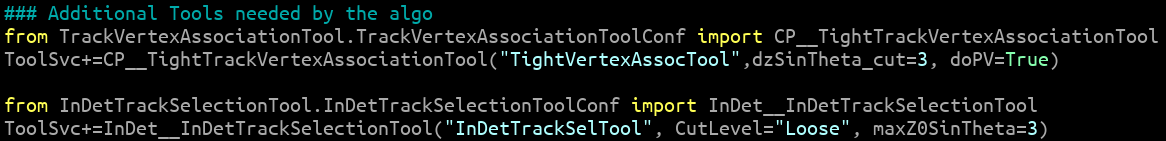
\includegraphics[width=\linewidth,height=\textheight,keepaspectratio]{cutlevel_screenshot}
    \end{figure}

\end{frame}
\frame{
    \frametitle{ MV2c10 Performance } 
    \begin{figure}
        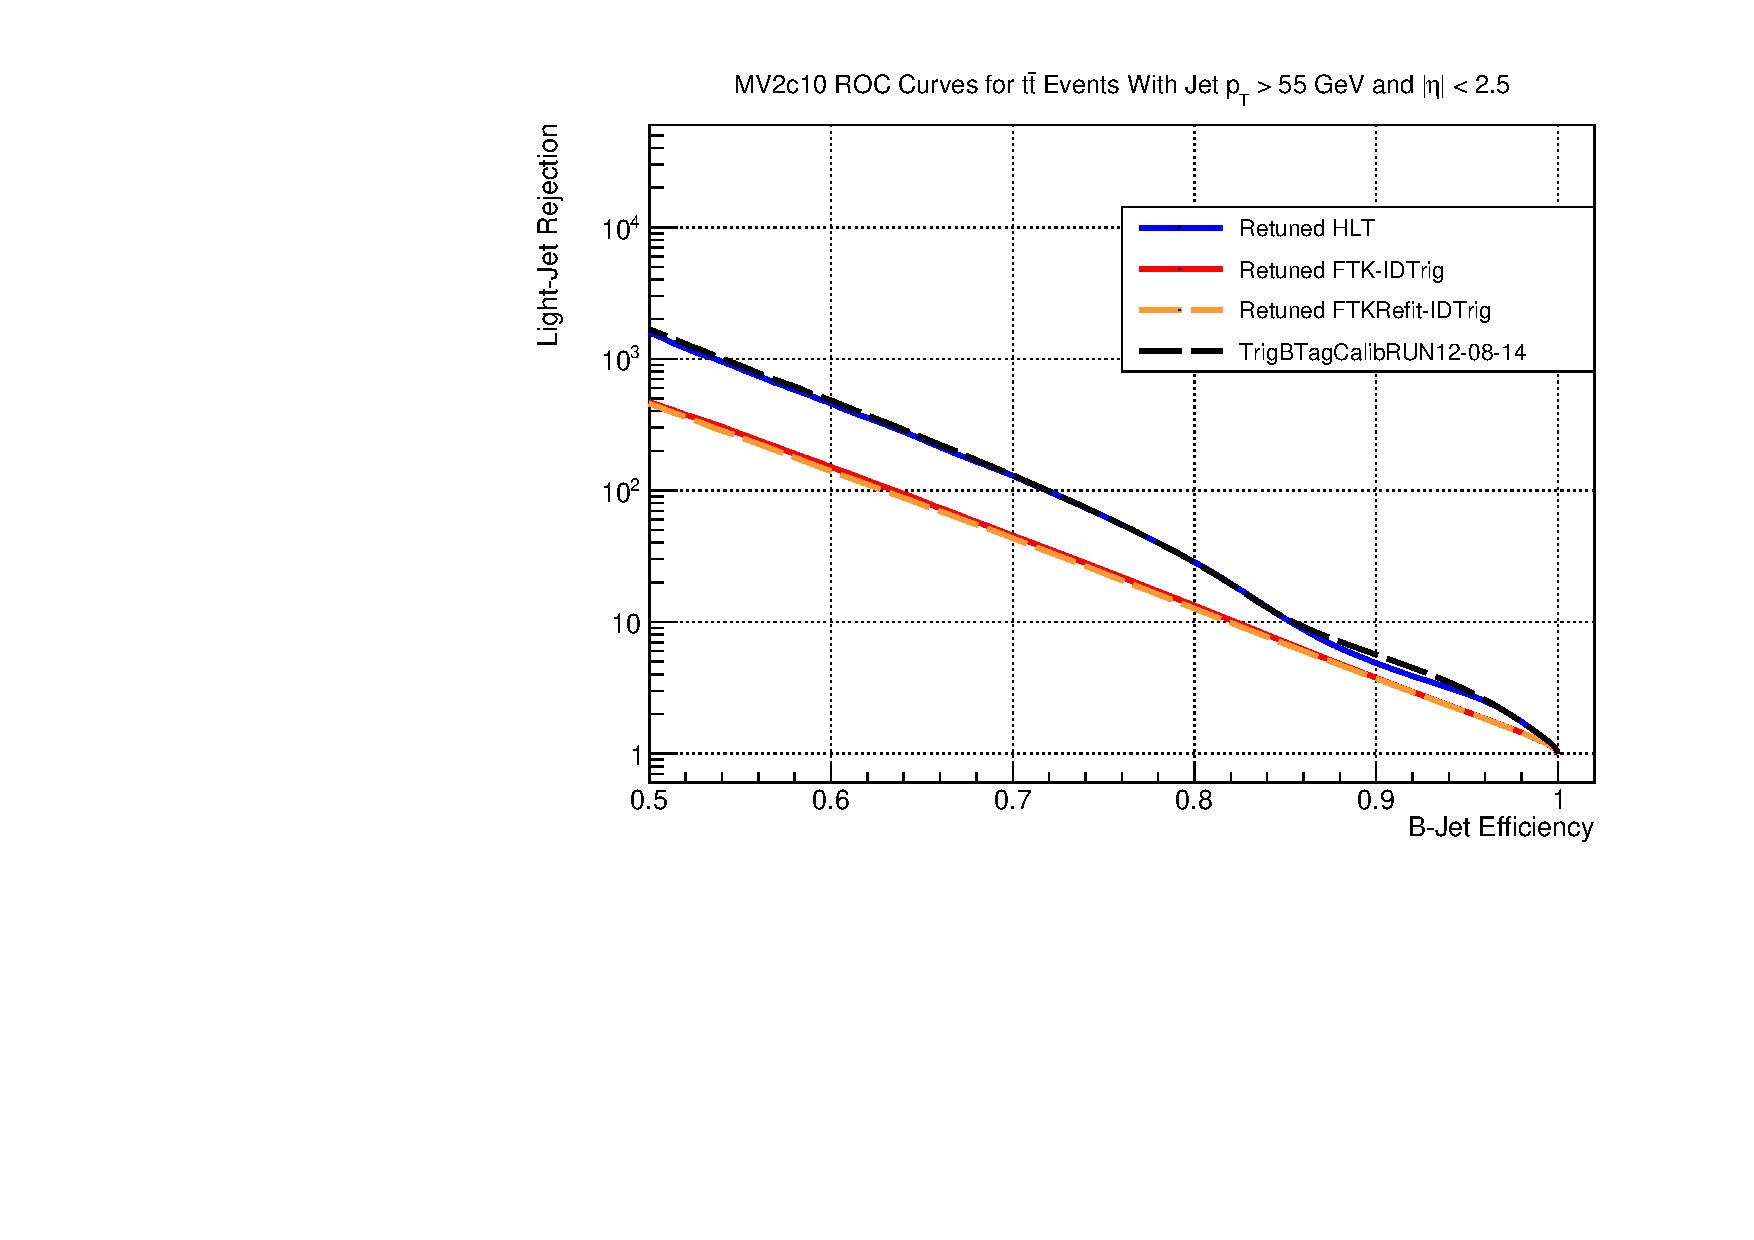
\includegraphics[width=\linewidth,height=\textheight,keepaspectratio]{btag_c10_score_comparison/mv2c10_roc_ttbar}
    \end{figure}
}
\frame{
    \frametitle{ IP2D and IP3D Performance } 
    \begin{columns}
        \begin{column}{0.5\textwidth}
            \begin{figure}
                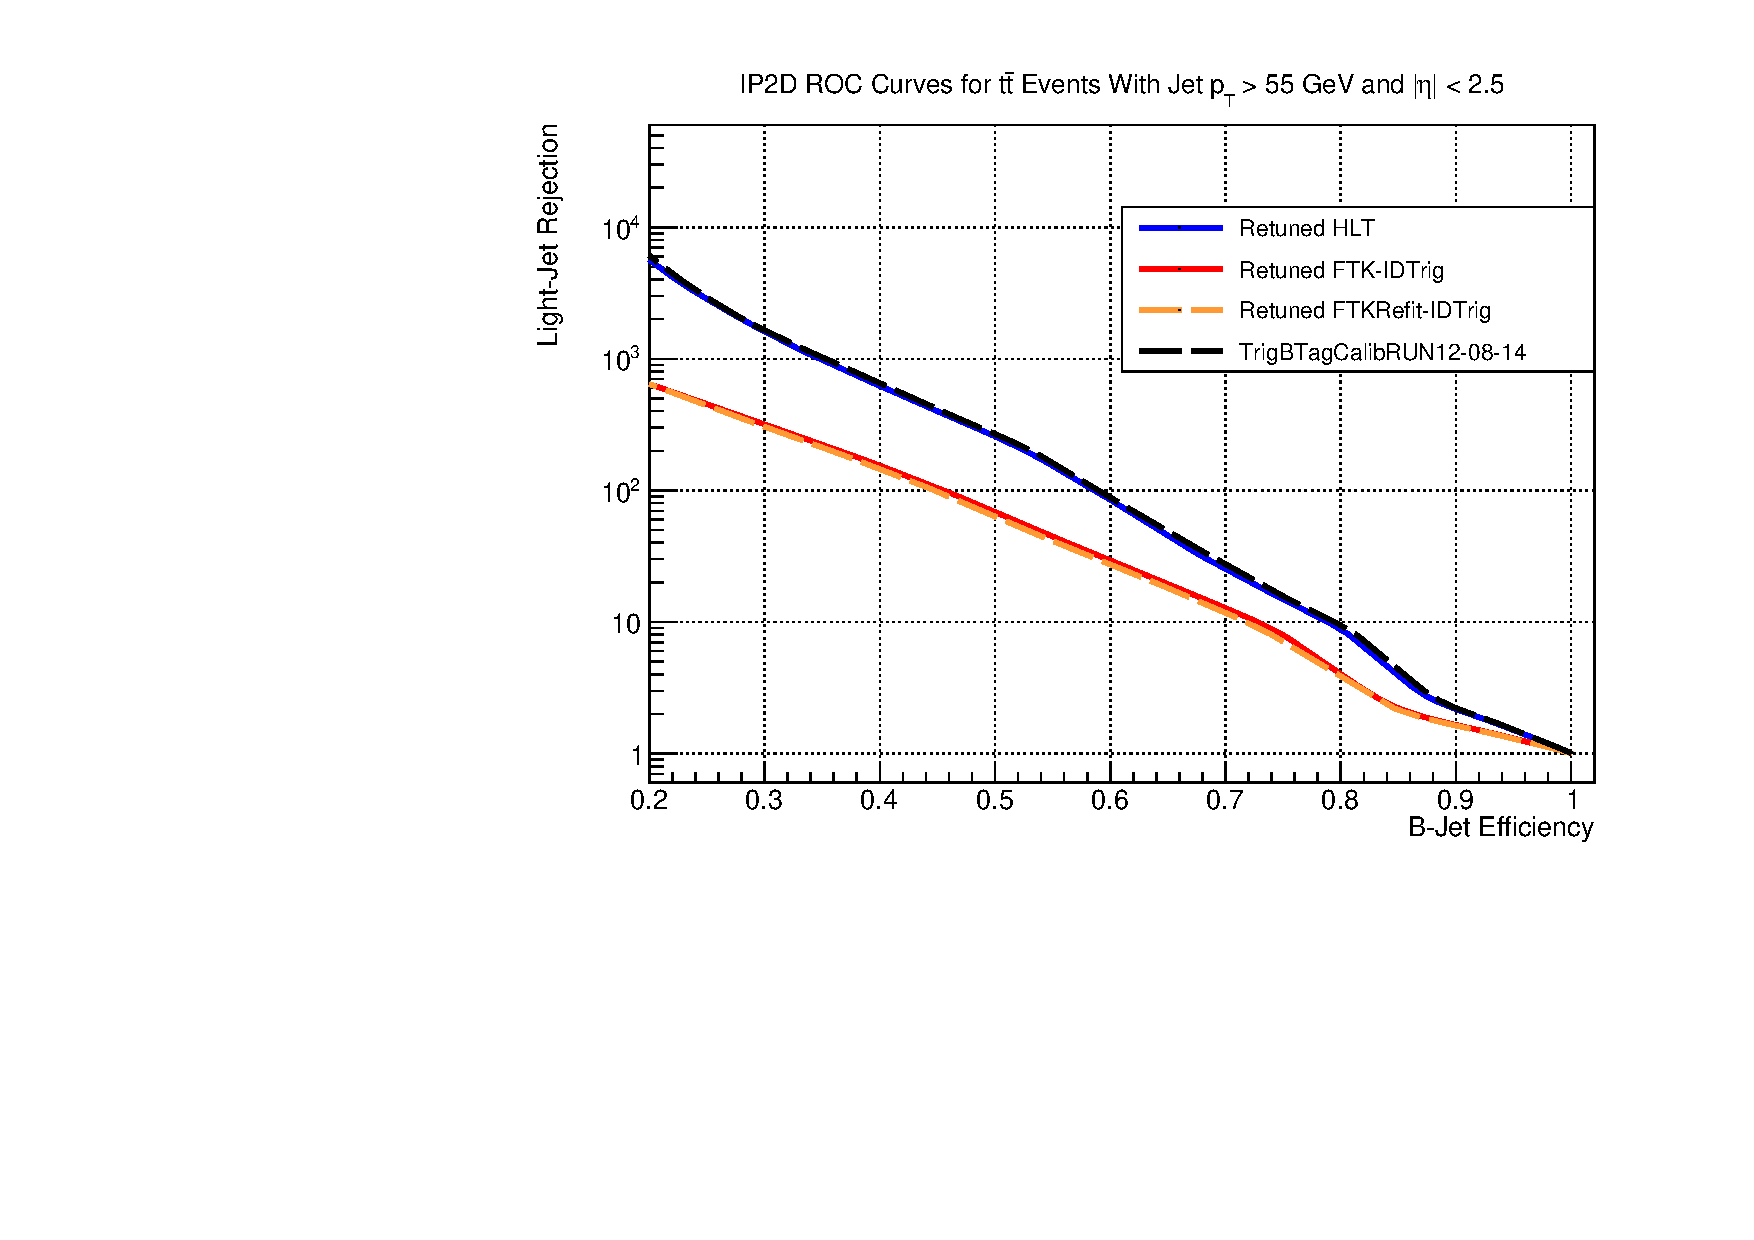
\includegraphics[width=\linewidth,height=\textheight,keepaspectratio]{ipxd_performance/performance_roc_ttbar_ip2d}
            \end{figure}
        \end{column}
        \begin{column}{0.5\textwidth}
            \begin{figure}
                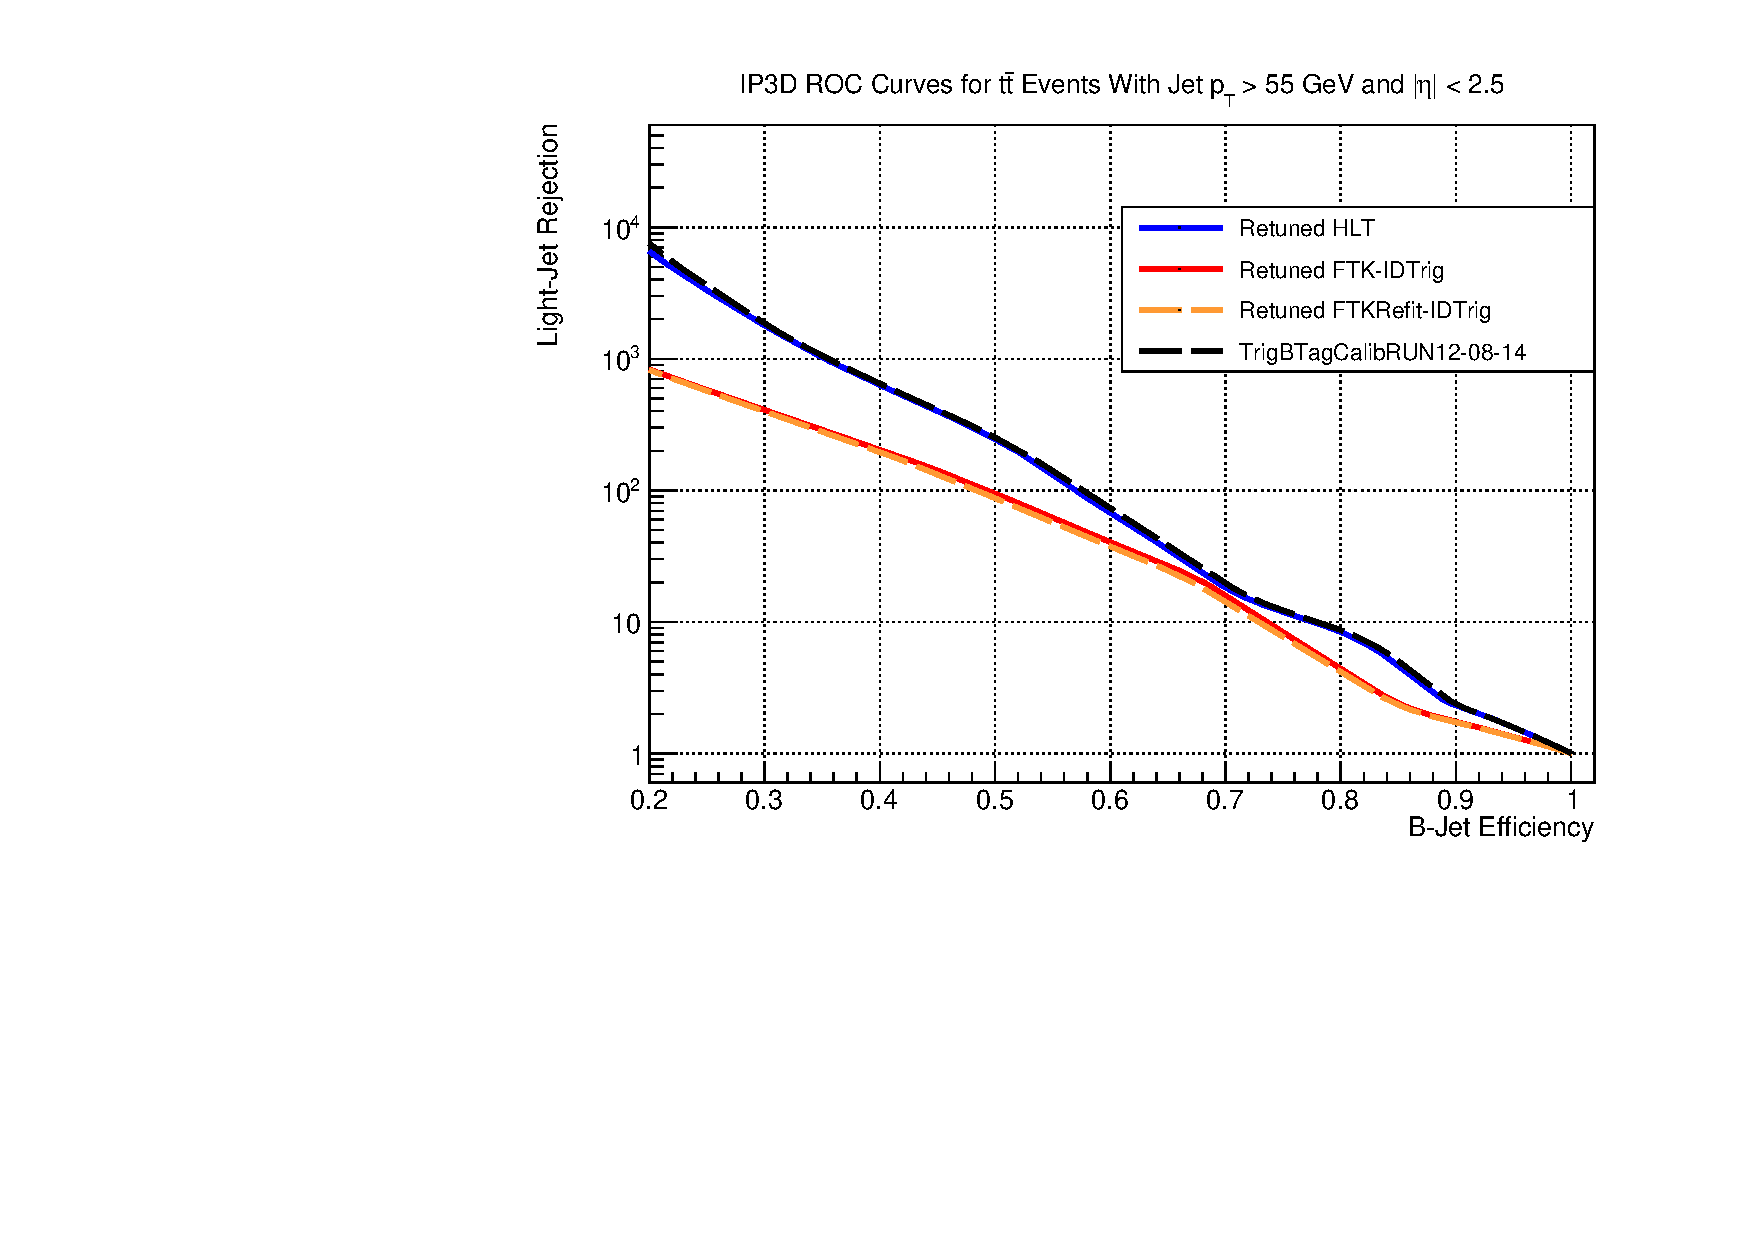
\includegraphics[width=\linewidth,height=\textheight,keepaspectratio]{ipxd_performance/performance_roc_ttbar_ip3d}
            \end{figure}
        \end{column}
    \end{columns}
}


